\documentclass{standalone}

\usepackage{tikz}
\usetikzlibrary{shapes.geometric}
\usetikzlibrary{arrows.meta}
\usetikzlibrary{intersections}
\usetikzlibrary{calc}

\newcommand\DrawDepot[1][black]{%
% #1: color
\tikzset{
    depot line/.style={
        line width=2pt,
        draw=black!80
    },
    depot fill/.style={
        fill=#1!80
    }
}
\def\NumItems{3}
\def\ItemSize{1}
\def\ItemSepX{0.5}
\def\ItemSepY{0.2}
\def\ItemMarginX{0.75}
\def\ItemMarginY{0.9}
\def\RoofAngle{30}
\def\BodyWidthX{1.5}
\def\BodyWidthY{0.65 * \BodyWidthX}
\pgfmathsetmacro{\InnerWidth}{%
    \NumItems * \ItemSize + (\NumItems - 1) * \ItemSepX + 2 * \ItemMarginX%
}
\pgfmathsetmacro{\InnerHeight}{%
    \NumItems * \ItemSize + (\NumItems - 1) * \ItemSepY + 2 * \ItemMarginY%
}
\pgfmathsetmacro{\OuterWidth}{%
    \InnerWidth + 2 * \BodyWidthX%
}
\pgfmathsetmacro{\OuterHeight}{%
    \InnerHeight + \BodyWidthY%
}
\pgfmathsetmacro{\RoofHeight}{%
    0.5 * \OuterWidth * tan(\RoofAngle)%
}

\coordinate (depot center) at (0, 0);

\path (depot center)
    ++ (-0.5*\OuterWidth, -0.5*\OuterHeight - 0.5*\RoofHeight)
    coordinate (depot south west);

\fill[depot fill]
    (depot south west)
    -- ++(\BodyWidthX, 0)
    -- ++(0, \InnerHeight)
    -- ++(\InnerWidth, 0)
    -- ++(0, -\InnerHeight)
    -- ++(\BodyWidthX, 0)
    -- ++(0, \OuterHeight)
    -- ++(-0.5*\OuterWidth, \RoofHeight)
    -- ++(-0.5*\OuterWidth, -\RoofHeight)
    -- cycle
    ;

\path (depot south west)
    ++ (\BodyWidthX + \ItemMarginX, 0.5*\ItemSepY)
    coordinate (depot current row south west)
    ;

\foreach \x in {1,...,\NumItems} {
    \pgfmathtruncatemacro{\NumItemsOnRow}{\NumItems - \x + 1}
    \path (depot current row south west)
        coordinate (depot current item south west)
        ;
    \foreach \y in {1,...,\NumItemsOnRow} {
        \draw[depot line, depot fill]
            (depot current item south west)
            rectangle ++(\ItemSize,\ItemSize)
            ;
        \path (depot current item south west)
            ++(0, \ItemSize + \ItemSepY)
            coordinate (depot current item south west)
            ;
    }
    \path (depot current row south west)
        ++(\ItemSize + \ItemSepX, 0)
        coordinate (depot current row south west)
        ;
}

\draw [-, depot line, name path=depot outline] 
    (depot south west)
    -- ++(\OuterWidth, 0)
    -- ++(0, \OuterHeight)
    -- ++(-0.5*\OuterWidth, \RoofHeight)
    -- ++(-0.5*\OuterWidth, -\RoofHeight)
    -- cycle
    ;

\draw[-, depot line, name path=depot inline] 
    (depot south west)
    ++(\BodyWidthX, 0)
    -- ++(0, \InnerHeight)
    -- ++(\InnerWidth, 0)
    -- ++(0, -\InnerHeight)
    ;

\draw[-, depot line]
    (depot south west)
    ++(0, \OuterHeight)
    -- ++(\OuterWidth, 0)
    ;
}

\newcommand\DrawCar[1][black]{%
% #1: color
\begin{tikzpicture}
\tikzset{
    car line/.style={
        line width=2pt,
        draw=black!80
    },
    car fill/.style={
        fill=#1!80
    }
}


\def\WheelRadius{0.5}
\def\WheelXSep{1.5}
\def\WheelMargin{0.1}
\pgfmathsetmacro{\WheelOuterRadius}{%
    \WheelRadius + \WheelMargin%
}
\def\HeadInnerWidth{0.9}
\def\HeadInnerHeight{0.8}
\pgfmathsetmacro{\HeadOuterWidth}{%
    \HeadInnerWidth + \WheelOuterRadius%
}
\def\TrunkMarginX{0.2}
\def\TrunkInnerHeight{2.5 * \HeadInnerHeight}
\pgfmathsetmacro{\TrunkOuterWidth}{%
    \WheelOuterRadius%
    + \WheelXSep%
    + 2 * \WheelOuterRadius%
    + \TrunkMarginX%
}
\pgfmathsetmacro{\TrunkOuterHeight}{%
    \TrunkInnerHeight + \WheelOuterRadius%
}

\path (0, 0)
    ++ ({-0.5 * \WheelXSep - \WheelOuterRadius}, {\WheelOuterRadius})
    coordinate (front wheel center)
    ++ ({\WheelXSep + 2 * \WheelOuterRadius}, 0)
    coordinate (rear wheel center)
    ;

\draw [car line, car fill]
    (front wheel center)
    circle (\WheelRadius)
    ;
\draw [car line, car fill]
    (rear wheel center)
    circle (\WheelRadius)
    ;

\draw [car line, car fill]
    (front wheel center)
    ++ ({\WheelOuterRadius}, 0)
    arc (0:90:{\WheelOuterRadius})
    -- ++(0, \TrunkInnerHeight)
    -- ++(\TrunkOuterWidth, 0)
    -- ++(0, -\TrunkOuterHeight)
    -- ++(-\TrunkMarginX, 0)
    arc (0:180:{\WheelOuterRadius})
    -- cycle
    ;

\draw [car line, car fill]
    (front wheel center)
    ++ (0, {\WheelOuterRadius})
    arc (90:180:{\WheelOuterRadius})
    [rounded corners=5pt]
    -- ++({-\HeadInnerWidth}, 0)
    -- ++(0, \HeadInnerHeight)
    -- ++(\HeadOuterWidth, \HeadInnerHeight)
    -- cycle
    ;

\end{tikzpicture}

}

\begin{document}

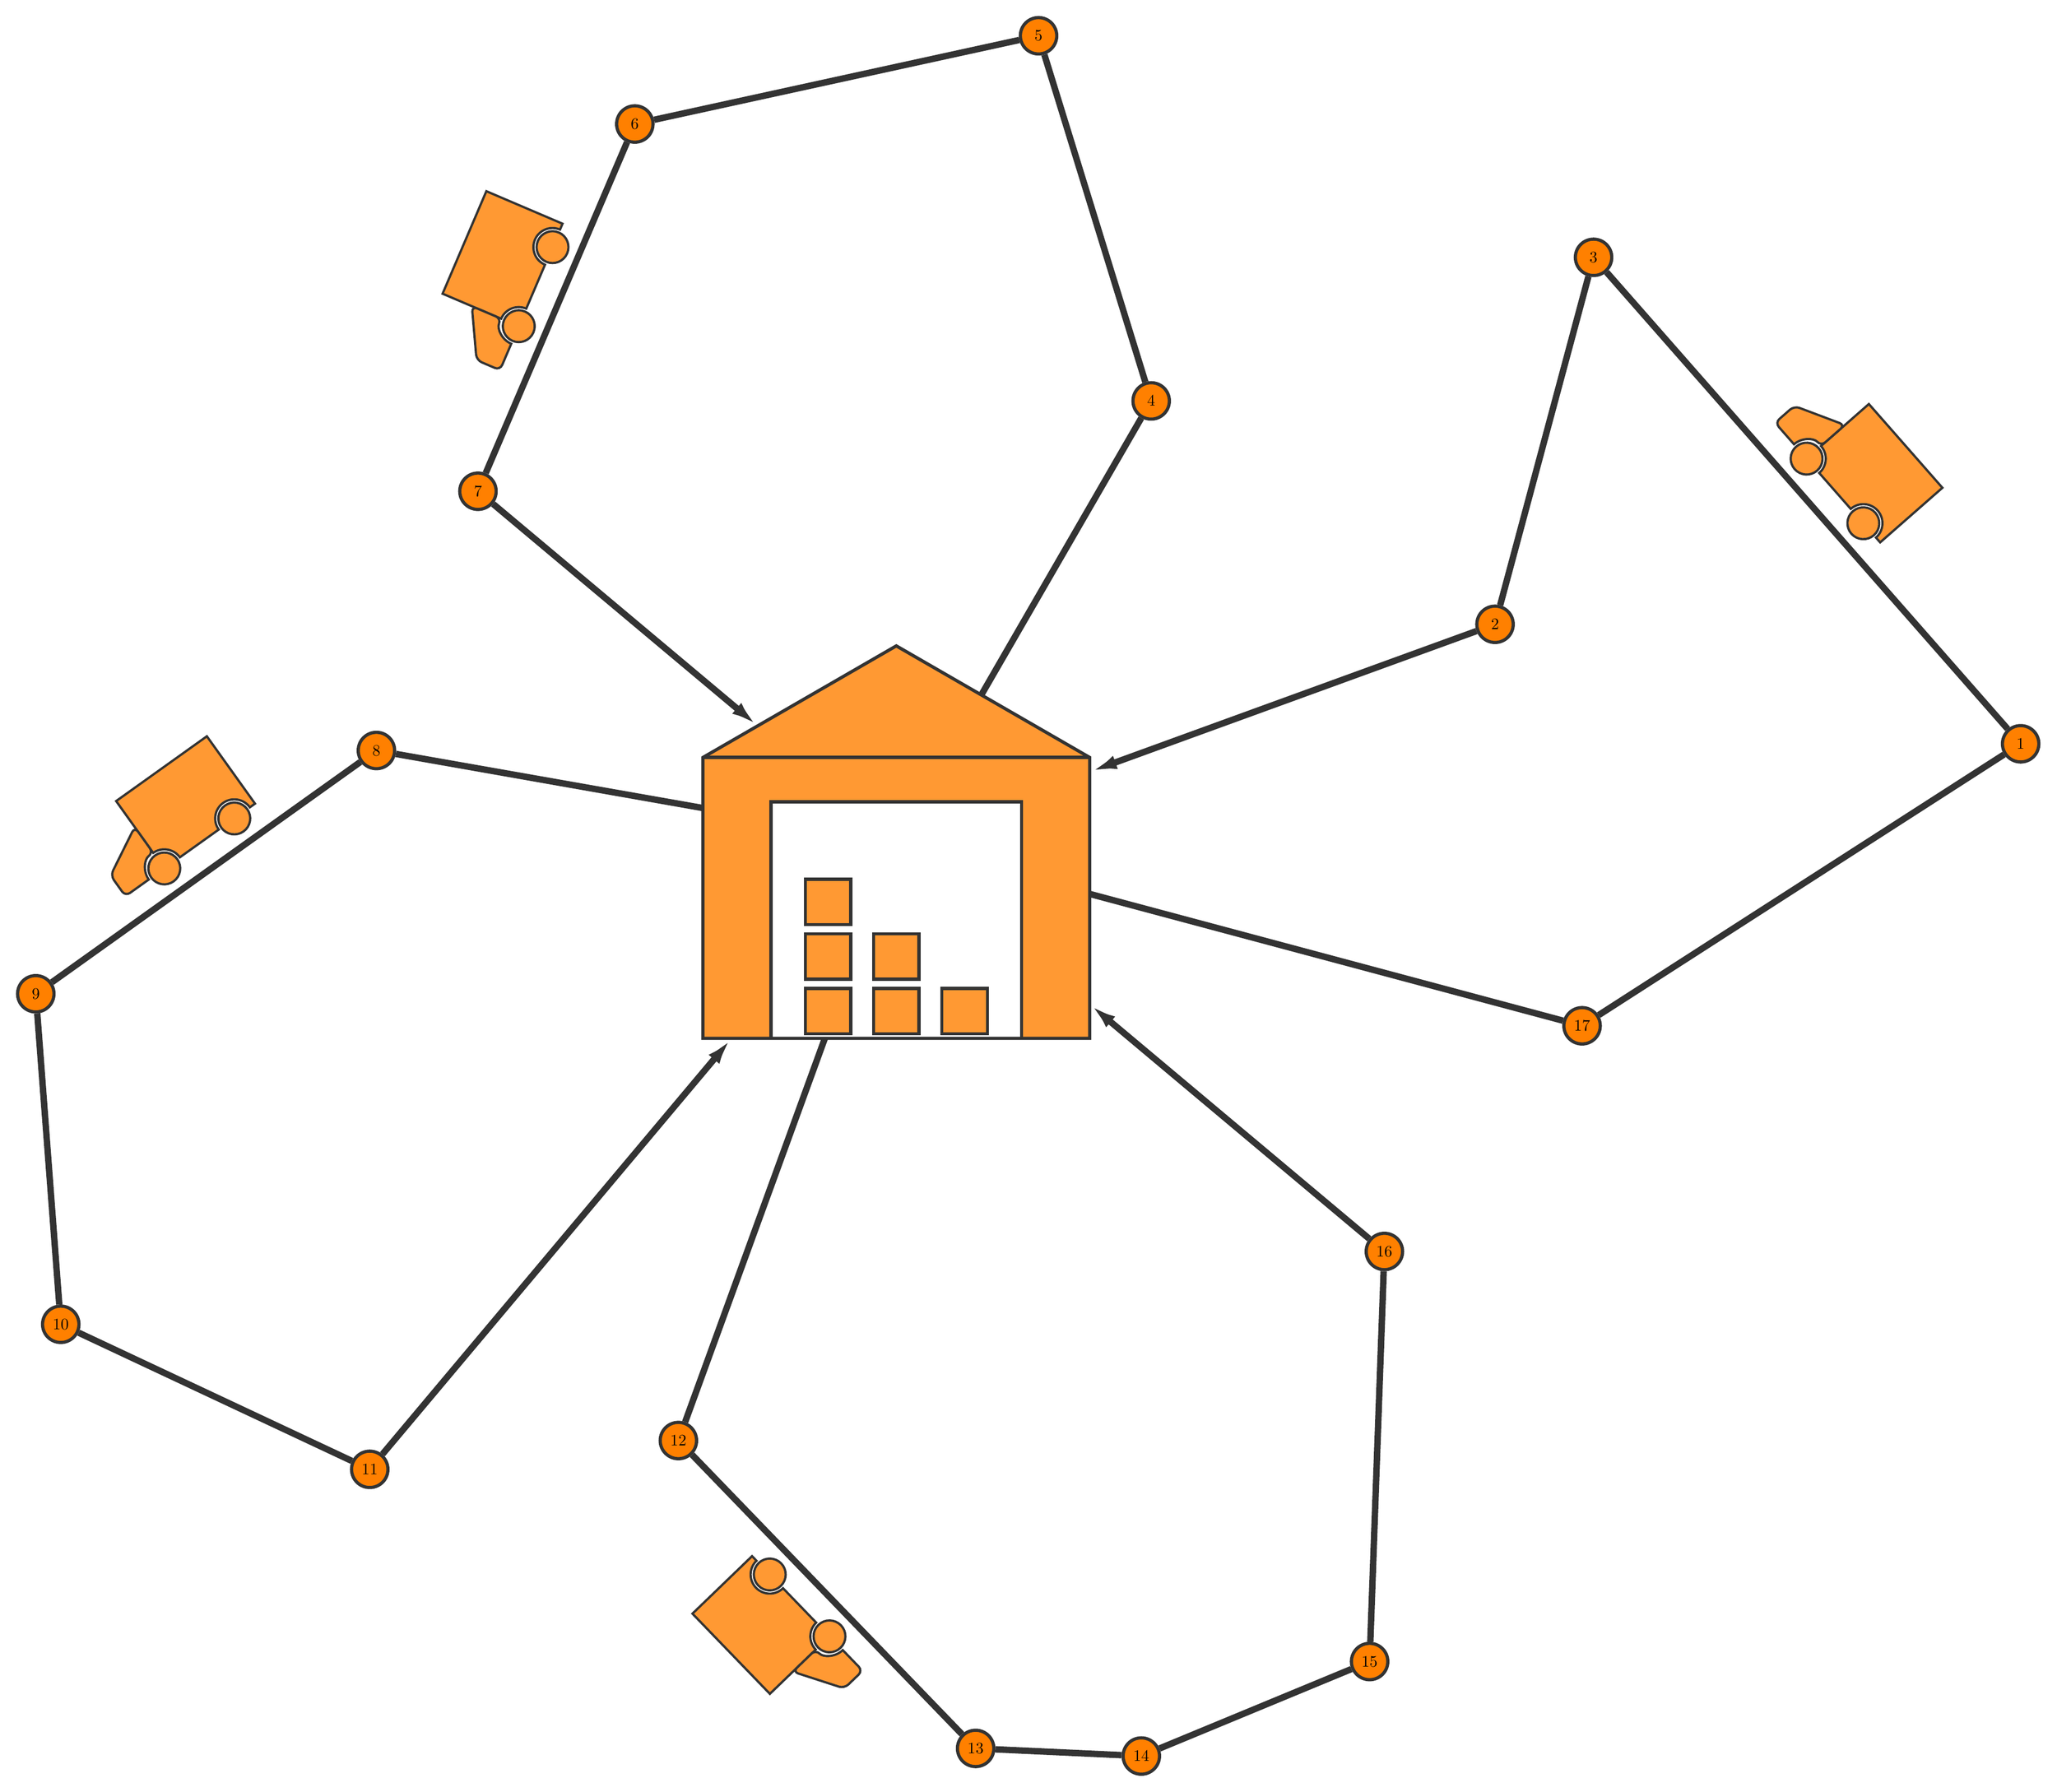
\begin{tikzpicture}

\DrawDepot[orange]

\tikzset{
    client/.style={
        circle,
        draw=black!80,
        fill=orange,
        minimum size=8mm,
        line width=2pt
    }
}

\def\Unit{4}

\foreach \Angle/\Radius [count=\i] in {%
    5/6.2,
    20/3.5,
    40/5,
    60/2.8,
    80/4.5,
    110/4.2,
    140/3,
    170/2.9,
    190/4.8,
    210/5.3,
    230/4.5,
    250/3.5,
    275/5,
    285/5.2,
    300/5.2,
    320/3.5,
    345/3.9%
} {
    \node[client] (client\i) at (\Angle:\Radius * \Unit) {};
}

\foreach \i in {1,...,17} {
    \node at (client\i) {\i};
}

% Routes:
% 2-3-1-17
% 4-5-6-7
% 8-9-10-11
% 12-13-14-15-16
\tikzset{
    route/.style={
        -{Latex[length=6mm, width=3mm]},
        line width=4pt,
        black!80
    }
}
\foreach \route in {%
    {17,1,3,2},
    {4,5,6,7},
    {8,9,10,11},
    {12,13,14,15,16}%
} {
    \def\Nodes{}
    \foreach \i [count=\c] in \route {
        \ifnum\c=1
            \xdef\FirstClient{\i}
            \xdef\Nodes{(client\i)}
        \else
            \xdef\Nodes{\Nodes -- (client\i)}
            \xdef\LastClient{\i}
        \fi
    }
    \path [name path=route start edge]
        (depot center) -- (client\FirstClient);
    \path [name path=route end edge]
        (client\LastClient) -- (depot center);
    \path[
        name intersections={%
            of=depot outline and route start edge,
            by=route start
        },
        name intersections={%
            of=depot outline and route end edge,
            by=route end
        }
    ];
    \draw[route] (route start) -- \Nodes -- (route end);
}

% Draw cars on edges
\foreach \startnode/\endnode/\angle in {%
    3/1/0,%
    6/7/0,%
    8/9/0,%
    12/13/180%
} {
    \path 
        (client\startnode)
        -- 
        node[
            pos=0.5,
            sloped,
            above,
            outer sep=4pt,
            rotate={\angle},
            scale=0.7
        ] {\DrawCar[orange]}
        (client\endnode)
        ;
}
\end{tikzpicture}

\end{document}